%template1.tex
%The following LaTeX source file represents the simplest kind of slide presentation; no overlays, no included graphics. Substitute your favorite style for ``pascal''. To create the PDF file template1.pdf, (1) be sure to use the prosper class, then (2) execute the command latex template1.tex, and (3) the command dvipdf template1.dvi.

%%%%%%%%%%%%%%%%%%%%%%%%%%%%%%% template1.tex %%%%%%%%%%%%%%%%%%%%%%%%%%%%%%%%%%%
\documentclass[a4paper,blends,pdf,colorBG,slideColor]{prosper}
% definitions for slides for CSC544
% Lutz Hamel, (c) 2007

\hypersetup{pdfpagemode=FullScreen}

\usepackage{times}
\usepackage{latexsym}
\usepackage{alltt}
\usepackage{booktabs}
\usepackage{amsmath}
\usepackage{amsopn}
\usepackage{amsfonts}
\usepackage{amssymb}
%\usepackage[usenames]{color}

\def\sign{\qopname\relax{no}{sign}}
\def\argmax{\qopname\relax{no}{argmax}}
\def\argmin{\qopname\relax{no}{argmin}}

\newcommand{\grad}{\ensuremath{\nabla}} 
\newcommand{\loss}{\ensuremath{{\cal L}}}
\newcommand{\err}{\mbox{err}}
\newcommand{\mse}{\mbox{mse}}
\newcommand{\acc}{\mbox{acc}}
\newcommand{\Integer}{\ensuremath{\mathbb{N}}}
\newcommand{\size}[1]{{|{#1}|}}
\newcommand{\Rnspace}[1]{\ensuremath{\mathbb{R}^{#1}}}
\newcommand{\Real}{\ensuremath{\mathbb{R}}}
\newcommand{\mytt}[1]{{\small\tt{#1}}}
\newcommand{\textemph}[1]{{\em #1}}
\newcommand{\suchthat}{\mid}
\newcommand{\orbar}{\;|\;}
\newcommand{\bs}[1]{\begin{slide}{#1}\ptsize{8}}
\newcommand{\es}{\end{slide}}
\newcommand{\co}{\,\colon\;}
\newcommand{\pair}[2]{\ensuremath{( {#1}, {#2} )}}
\newcommand{\model}[1]{\hat{#1}}
\newcommand{\ul}[1]{{\bf\em #1}}
\newcommand{\ol}{\overline}
\newcommand{\definition}[1]{{\bf Definition: }{\em #1}}
\newcommand{\example}[1]{{\bf Example: }{#1}}
\newcommand{\abs}[1]{|{#1}|}
\newcommand{\mytab}{\makebox[.1in]{}}

\newcommand{\fdef}[1]{
\begin{center}
\fbox{
\begin{minipage}{3.5in}
{\bf Definition:}
{#1}
\end{minipage}
}
\end{center}
}

\newcommand{\fframe}[1]{
\begin{center}
\fbox{
\begin{minipage}{3.5in}
{#1}
\end{minipage}
}
\end{center}
}

\newcommand{\nframe}[1]{
\begin{center}
\begin{minipage}{3.5in}
{#1}
\end{minipage}
\end{center}
}

\newenvironment{Rcode}
	{
		\scriptsize
		\begin{quote}
		\begin{alltt}
	}
	{
		\end{alltt}
		\end{quote}
	}




\begin{document}


\bs{\large Dual Maximum Margin Optimization}

{\bf Observations:}

\begin{itemize}
\item Support vector machines can be viewed as the dual to maximum margin classifiers.
\item We derive this dual representation using Lagrangian optimization theory.
\end{itemize}
\es

\bs{\large Dual Maximum Margin Optimization}
Assume that we are given a linearly separable training set of the following form,
\begin{equation*}
D = \{(\ol{x}_1,y_1),(\ol{x}_2,y_2),\ldots,(\ol{x}_l,y_l)\} \subseteq \Rnspace{n}\times\{+1, -1\},
\end{equation*}
then recall our primal maximum margin optimization problem,
\begin{gather*}
\min_{\ol{w},b}\phi(\ol{w},b) =\min_{\ol{w},b}\frac{1}{2}\ol{w}\bullet\ol{w},\\
\intertext{subject to the constraints,}
g_i(\ol{w},b) = y_i(\ol{w}\bullet\ol{x}_i -b) - 1\ge 0,
\end{gather*}
for $i = 1,\ldots,l$.

The constraints are rewritten in a form amenable for the Lagrangian objective function.

\es

\bs{\large Dual Maximum Margin Optimization}

We construct the corresponding Lagrangian as,
\begin{equation*}
\begin{aligned}
L(\ol{\alpha},\ol{w},b) &=  \phi(\ol{w},b) - \sum_{i=1}^l \alpha_i g_i(\ol{w},b) \\
& =  \frac{1}{2}\,\ol{w}\bullet\ol{w} - \sum_{i=1}^l \alpha_i (y_i(\ol{w}\bullet\ol{x}_i-b) - 1)\\
& =  \frac{1}{2}\,\ol{w}\bullet\ol{w} 
	- \sum_{i=1}^l \alpha_i y_i\ol{w}\bullet\ol{x}_i
	+ b\sum_{i=1}^l \alpha_i y_i
	+ \sum_{i=1}^l \alpha_i.
\end{aligned}
\end{equation*}
This gives us the Lagrangian optimization problem for maximum margin classifiers,
\begin{gather*}
\max_{\ol{\alpha}} \min_{\ol{w},b} L(\ol{\alpha},\ol{w},b) ,\\
\intertext{subject to,}
\alpha_i \ge 0,
\end{gather*}
for $i = 1, \ldots, l$.
\es


\bs{\large Dual Maximum Margin Optimization}
Now, let $\ol{\alpha}^*$, $\ol{w}^*$, and $b^*$ be a solution to the Lagrangian optimization problem
such that,
\begin{equation*}
\max_{\ol{\alpha}} \min_{\ol{w},b} L(\ol{\alpha},\ol{w},b) = L(\ol{\alpha}^*,\ol{w}^*,b^*).
\end{equation*}
But,
\begin{itemize}
\item $\phi$ is convex
\item the constraints $g_i$ are linear
\end{itemize}
this implies that the solution
 $\ol{\alpha}^*$, $\ol{w}^*$ and $b^*$ will satisfy
the following KKT conditions,
\begin{align*}
\frac{\partial L}{\partial \ol{w}}(\ol{\alpha}^*, \ol{w}^*, b^*) &= \ol{0},\\
\frac{\partial L}{\partial b}(\ol{\alpha}^*, \ol{w}^*, b^*) &= 0,\\
\alpha^*_i (y_i(\ol{w}^*\bullet\ol{x}_i -b^*) - 1) &= 0,\\
y_i(\ol{w}^*\bullet\ol{x}_i -b^*) - 1 &\ge 0,\\
\alpha_i^* &\ge 0,
\end{align*}
for $i = 1,\ldots,l$.
\es

\bs{\large Dual Maximum Margin Optimization}
Of particular interest is of course the third condition,
\[
\alpha^*_i (y_i(\ol{w}^*\bullet\ol{x}_i -b^*) - 1) = 0,
\]
the complimentarity condition, because it assures the existence of a solution to our primal 
maximum margin optimization problem,
\begin{align*}
\max_{\ol{\alpha}} \min_{\ol{w},b} L(\ol{\alpha},\ol{w},b) &= L(\ol{\alpha}^*,\ol{w}^*,b^*) \\
&= \frac{1}{2}\,\ol{w}^*\bullet\ol{w}^* - \sum_{i=1}^l \alpha^*_i (y_i(\ol{w}^*\bullet\ol{x}_i-b^*) - 1)\\
&=\frac{1}{2}\,\ol{w}^*\bullet\ol{w}^*\\
&= \phi(\ol{w}^*,b^*).
\end{align*}
\es

\bs{\large Dual Maximum Margin Optimization}
\small
As in our simple, one dimensional example we want to solve the Lagrangian optimization problem
by constructing and solving the Lagrangian dual.

In order to accomplish this we first construct expressions for the optima of the primal variables 
at the saddle point.  We know that they exist because of the KKT conditions.  Therefore,
\begin{equation*}
\frac{\partial L}{\partial \ol{w}} (\ol{\alpha},\ol{w}^*,b)=
	\ol{w}^* - \sum_{i=1}^l \alpha_i y_i  \ol{x}_i = \ol{0}.
\end{equation*}
It follows that,
\begin{equation*}
\ol{w}^* = \sum_{i=1}^l \alpha_i y_i  \ol{x}_i.
\end{equation*}
And also,
\begin{equation*}
\frac{\partial L}{\partial b}  (\ol{\alpha},\ol{w},b^*)= \sum_{i=1}^l \alpha_i y_i  = 0,
\end{equation*}
giving rise to the constraint
\begin{equation*}
 \sum_{i=1}^l \alpha_i y_i  = 0,
\end{equation*}
that needs to hold at the saddle point.
\es

\bs{\large Dual Maximum Margin Optimization}
\small
{\bf Observation:} No expression for $b^*$!

However, we can recover an expression for $b^*$ from the structure of the data set.
\begin{center}
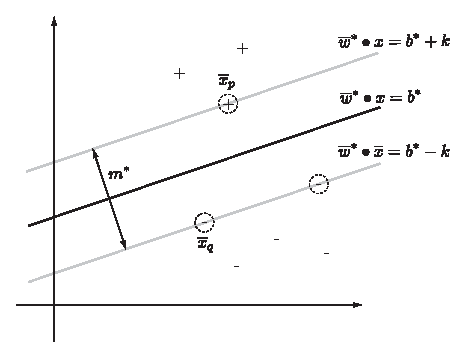
\includegraphics[height=35mm]{figures/fig06-05.eps}
\end{center}
\begin{minipage}{2.2in}
\scriptsize
\begin{gather*}
b^+ = \ol{w}^*\bullet\ol{x}_p\\
\intertext{or computationally,}
b^+ = \min \{\ol{w}^*\bullet\ol{x} \mid (\ol{x},y)\in D \text{ with } y = +1\}
\end{gather*}
\end{minipage}
\begin{minipage}{1.8in}
\small
\begin{gather*}
b^- = \ol{w}^*\bullet\ol{x}_q\\
\intertext{again computationally,}
b^- = \max\{\ol{w}^*\bullet\ol{x} \mid (\ol{x},y)\in D \text{ with } y = -1\}
\end{gather*}
\end{minipage}
\es


\bs{\large Dual Maximum Margin Optimization}

\vspace{.2in}
Now, the decision surface with $b^*$ as an offset sits right in the middle of the margin between the
two supporting hyperplanes, therefore
\begin{equation*}
\label{eq:b-value}
b^* = \frac{b^+ + b^-}{2}.
\end{equation*}
\es

\bs{\large Dual Maximum Margin Optimization}
\vspace{.2in}
We are now ready to construct our Lagrangian dual,
\begin{equation*}
 \phi'(\ol{\alpha}) =  L(\ol{\alpha},\ol{w}^*, b^*) 
 =  \sum_{i=1}^l \alpha_i - 
  \frac{1}{2}\sum_{i=1}^l\sum_{j=1}^l \alpha_i \alpha_j y_i y_j \ol{x}_i \bullet \ol{x}_j,
\end{equation*}
by applying the identity for $\ol{w}^*$ and the newly found constraint to the Lagrangian.
\es


\bs{\large Dual Maximum Margin Optimization}
\fframe{{\bf Proposition:}
(The Maximum Margin Lagrangian Dual)
Given the primal maximum margin optimization, \footnote{See lecture notes on maximum margin
classifiers.}
then the Lagrangian dual optimization for maximum margin classifiers is
\begin{equation*}
\max_{\ol{\alpha}} \phi'(\ol{\alpha}) = 
  \max_{\ol{\alpha}} \left ( \sum_{i=1}^l \alpha_i - 
  \frac{1}{2}\sum_{i=1}^l \sum_{j=1}^l \alpha_i \alpha_j y_i y_j \ol{x}_i \bullet \ol{x}_j \right ),
\end{equation*}
subject to the constraints
\begin{align*}
\sum_{i=1}^l \alpha_i  y_i &= 0,\\
\alpha_i  &\ge 0, 
\end{align*}
with $i = 1,\ldots,l$.
}
\es

\bs{\large Dual Maximum Margin Optimization}
\small
Given a solution $\ol{\alpha}^*$ to the Lagrangian dual optimization,
then the KKT complementarity condition  can only be satisfied for each $i = 1,\ldots,l$ if either $\alpha^*_i = 0$ or
$y_i(\ol{w}^*\bullet\ol{x}_i-b^*)-1 = 0$.  

If we consider $\alpha^*_j > 0$ for some point $(\ol{x}_j,y_j)\in D$, then 
in order to satisfy the complementarity condition we have
$y_j(\ol{w}^*\bullet\ol{x}_j-b^*) - 1 = 0$ or,
\begin{align*}
\ol{w}^*\bullet\ol{x}_j & = b^* + 1 \quad\text{ if $y_j = +1$},\\
\ol{w}^*\bullet\ol{x}_j & = b^* - 1 \quad\text{ if $y_j = -1$}.
\end{align*}
That is, the point $(\ol{x}_j,y_j)$ lies on one of the supporting hyperplanes!  It is a constraint!

Now consider $\alpha^*_j = 0$ for some point $(\ol{x}_j,y_j)\in D$.
That is, the point $\ol{x}_j$ is a point that does not lie in the vicinity of the class boundary
because we have $y_j(\ol{w}^*\bullet\ol{x}_j-b^*) - 1 > 0$ or,
\begin{align*}
\ol{w}^*\bullet\ol{x}_j & > b^* + 1 \quad\text{ if $y_j = +1$},\\
\ol{w}^*\bullet\ol{x}_j & < b^* - 1 \quad\text{ if $y_j = -1$}.
\end{align*}
This implies that points with zero-valued Lagrangian multipliers do not constrain the size of the 
margin.

\begin{center}
\fbox{Points with non-zero Lagrangian multipliers are support vectors!}
\end{center}
\es

\bs{\large Dual Maximum Margin Optimization}
This gives us the following insight,
\fframe{
The primal maximum margin optimization computes the supporting hyperplanes whose margin is limited by support vectors. 
The dual maximum margin optimization computes the support
vectors that limit the size of the margin of the supporting hyperplanes.
}
\vspace{.2in}
\begin{center}
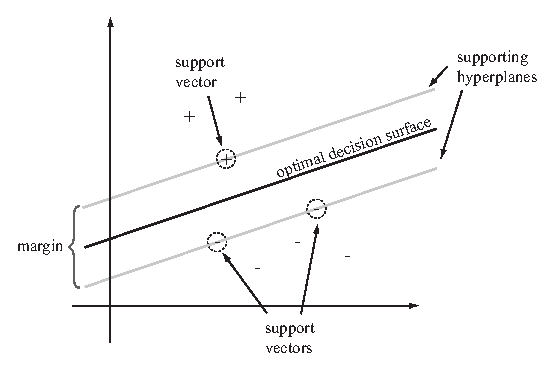
\includegraphics[height=40mm]{figures/fig06-03.eps}
\end{center}


\es
\end{document}
%%%%%%%%%%%%%%%%%%%%%%%%%%% end of template1.tex %%%%%%%%%%%%%%%%%%%%%%%%%%%%%%%%

